Suppose we have a set of pre-classified data points $x_i$ in $\mathbb{R}^n$, divided into two sets based on their classification. For example, the data could be information on patients and the two sets would correspond to patients who have or do not have a certain disease. Note that unlike so far, $x$ is now data, not a decision variable. Denote the respective index sets by $I_1$ and $I_2$, respectively. In order to predict the class of a new point $x_{new}$, we want to infer a classification rule from the data.

\begin{figure}[H]
    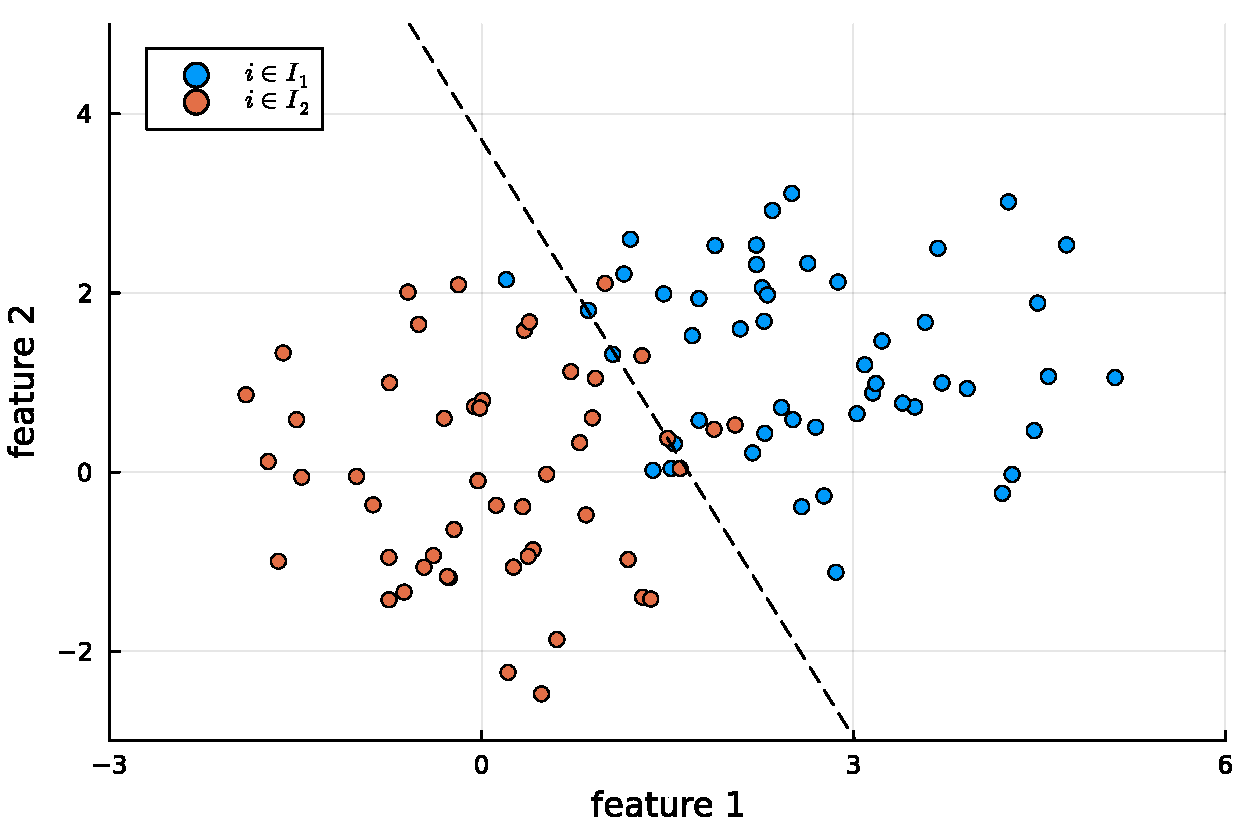
\includegraphics[width=0.75\textwidth]{chapters/chapter_1/figures/figure_e16.pdf}
    \caption{Two sets of data points defined by two features, separated by a line $ax=b$} 
    \label{c1:fig:fig_e16}		
\end{figure}

Write a linear programming problem that finds the hyperplane $a^\top x = b$ such that if $a^\top x_{new} > b$, the point $x_{new}$ is predicted to be in class 1, and if $a^\top x_{new}<b$, the predicted class is 2. The hyperplane should be optimal in the sense that it minimises the sum of absolute deviations $|a^\top x_i-b|$ for the misclassified points $x_i$ in the training data, that is, points on the wrong side of the hyperplane. In Figure \ref{c1:fig:fig_e16}, any orange point $x_i$, $i \in I_2$ that is on the top/right of the line is on the wrong side and thus accumulates the error, and similarly for blue points on the bottom/left of the line.
